\section{PROCEDIMIENTO} 

\begin{itemize}
\subsection{ACTIVIDAD 01}
	\subsubsection{Importación de Datos usando el Wizard - SQL MANAGMENT}

	\item Primero hay que crear una base de datos llamada BDTEST.

	\begin{center}
	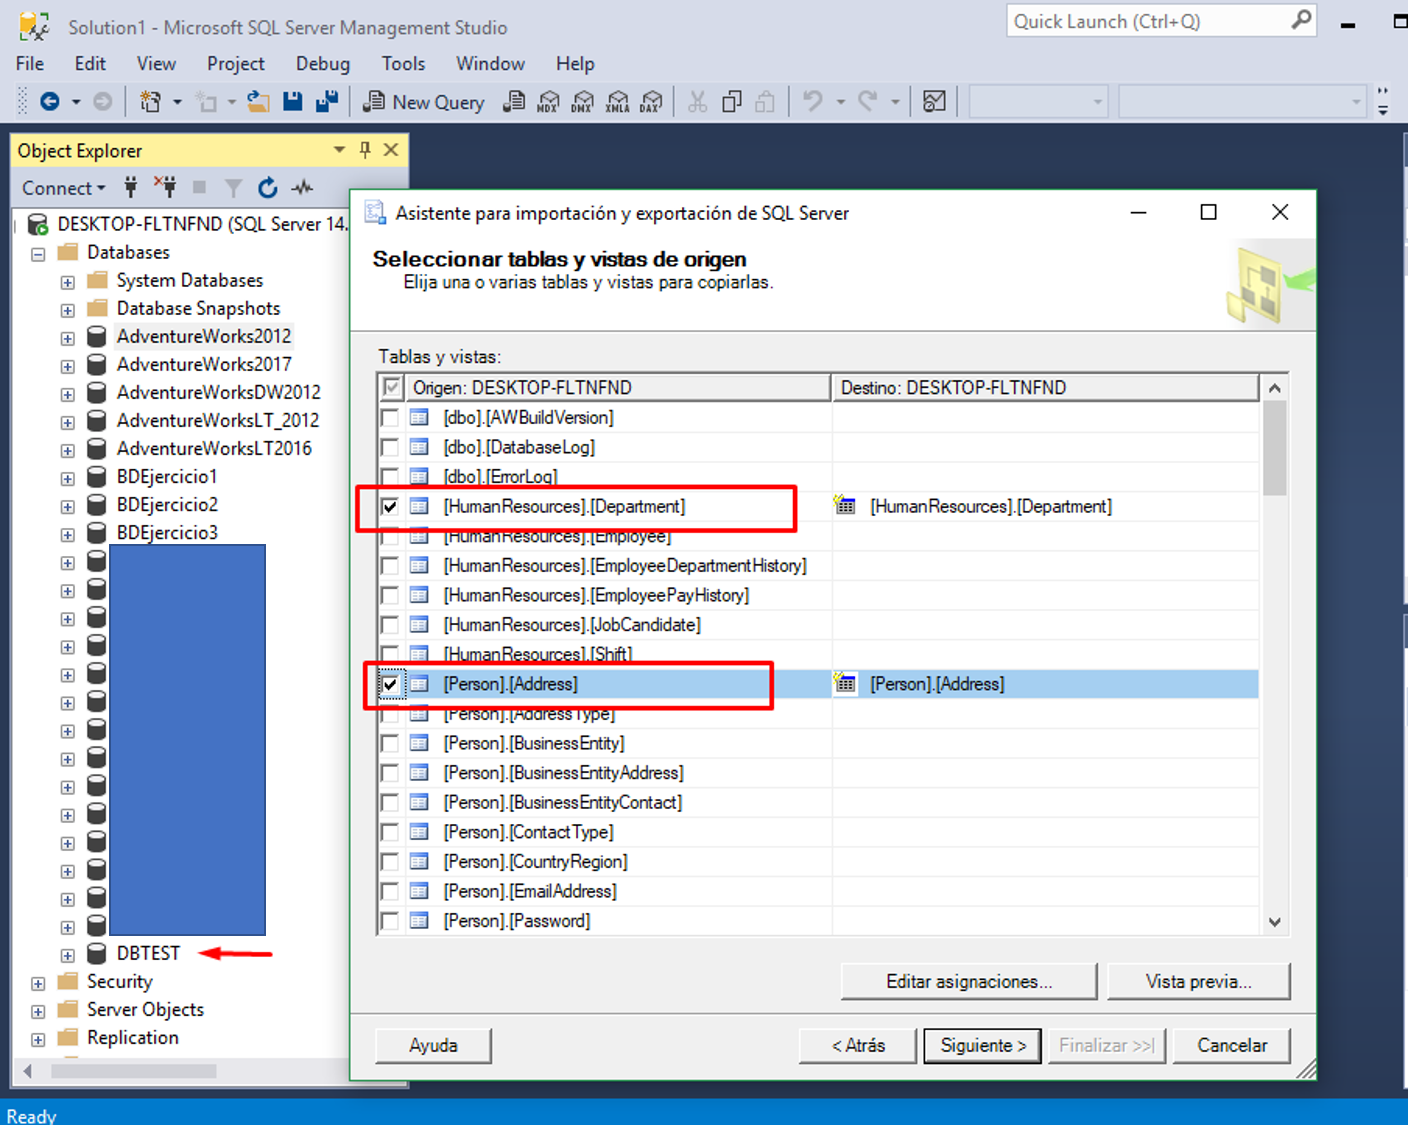
\includegraphics[width=14cm]{./Imagenes/tarea1}
	\end{center}
	
	\item  Ahora importaremos nuestra base de datos desde AdventureWorks.
	\begin{center}
	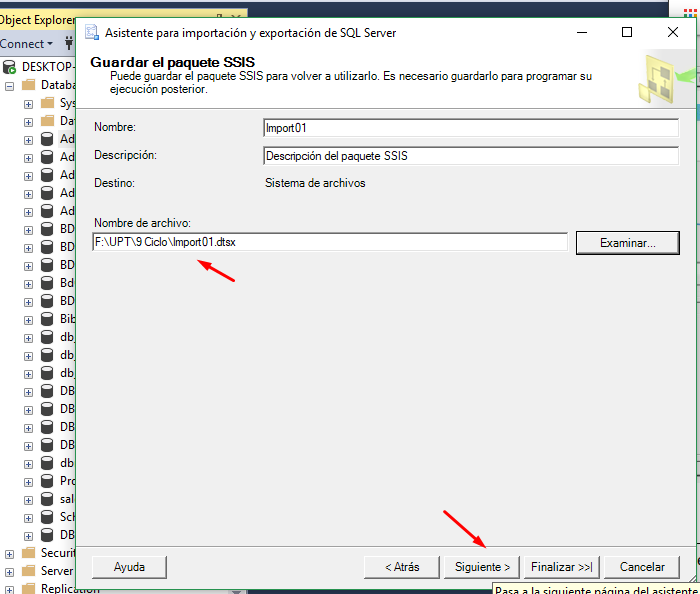
\includegraphics[width=14cm]{./Imagenes/tarea1_2}
	\end{center}

\begin{center}
	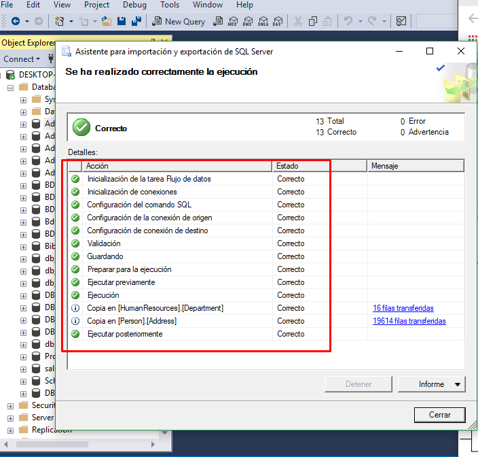
\includegraphics[width=14cm]{./Imagenes/tarea1_3}
	\end{center}
\begin{center}
	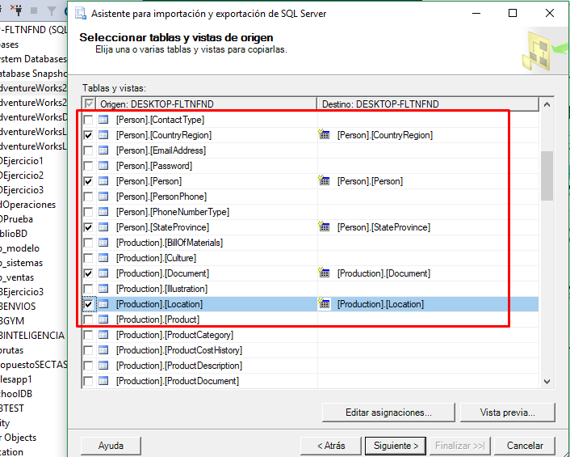
\includegraphics[width=14cm]{./Imagenes/tarea1_4}
	\end{center}
\begin{center}
	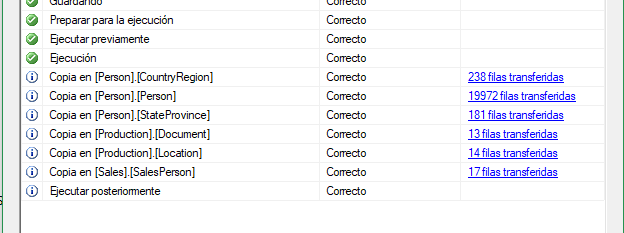
\includegraphics[width=14cm]{./Imagenes/tarea1_5}
	\end{center}

\subsection{ACTIVIDAD 02}

\subsubsection{Creación del primer paquete DTSX}

		\item Abriremos un Proyecto nuevo en Visual Studio

	\begin{center}
	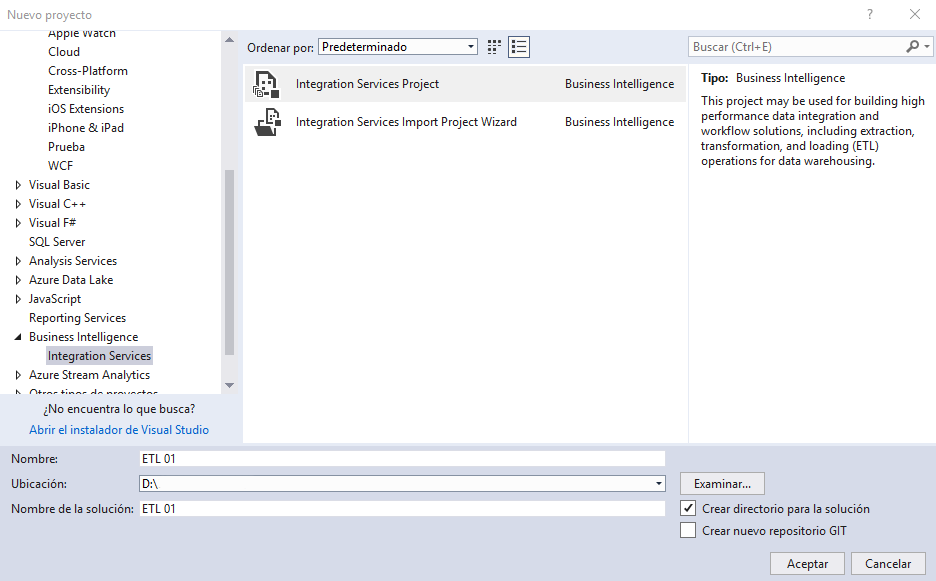
\includegraphics[width=14cm]{./Imagenes/tarea2_1}
	\end{center}

\item En la ventana nueva, sección Solución Explorer, Agrego el paquete generado antes.

	\begin{center}
	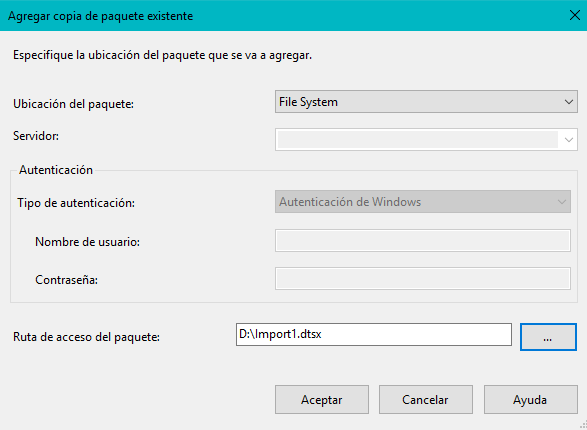
\includegraphics[width=14cm]{./Imagenes/tarea2_2}
	\end{center}

	\begin{center}
	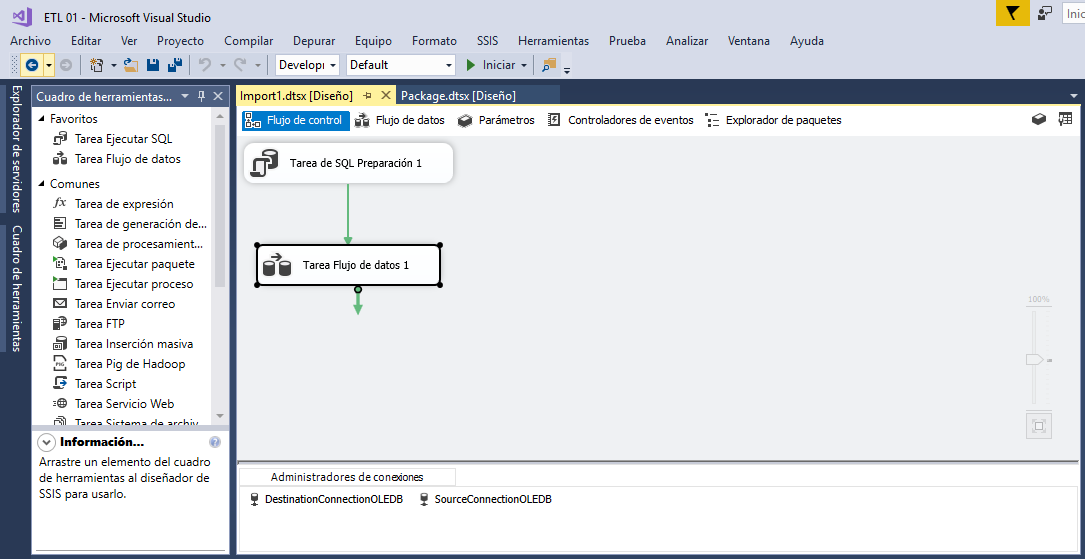
\includegraphics[width=14cm]{./Imagenes/tarea2_3}
	\end{center}

	\begin{center}
	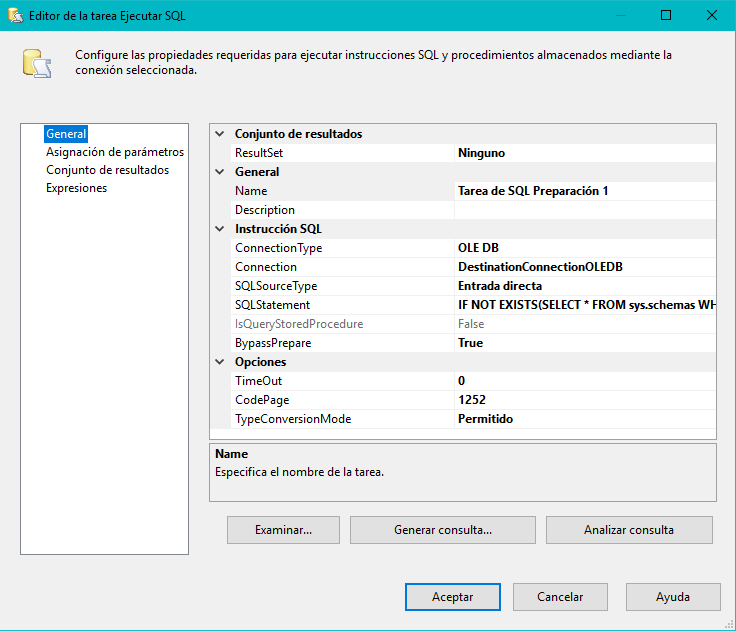
\includegraphics[width=14cm]{./Imagenes/tarea2_4}
	\end{center}

\item  En la siguiente ventana mostramos el paquete que se ha importado

	\begin{center}
	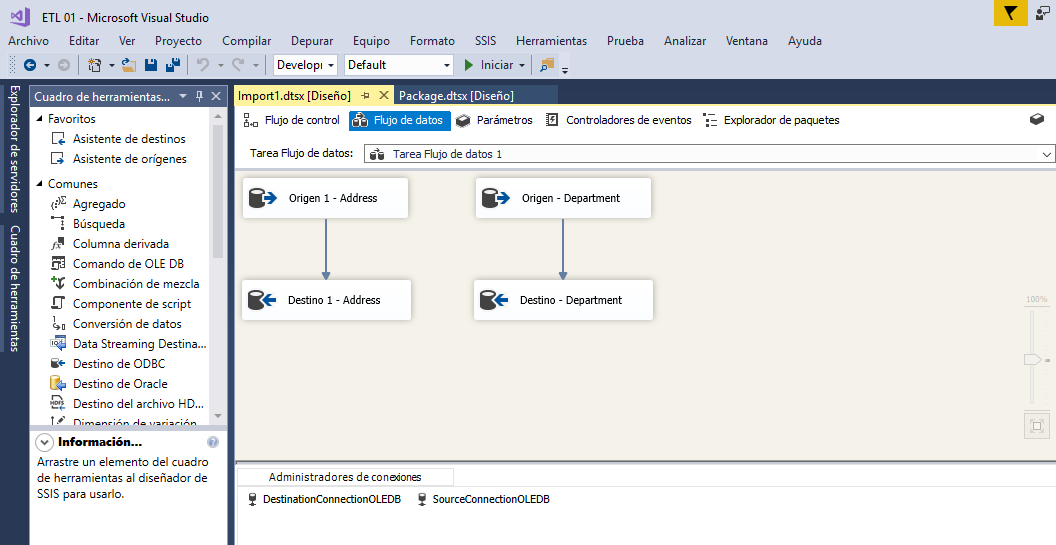
\includegraphics[width=14cm]{./Imagenes/tarea2_5}
	\end{center}
	\begin{center}
	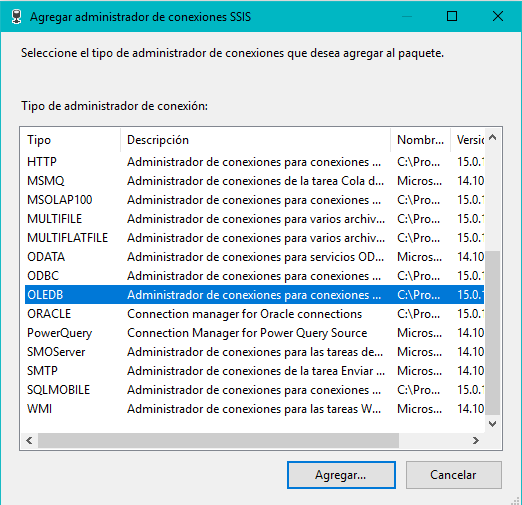
\includegraphics[width=14cm]{./Imagenes/tarea2_6}
	\end{center}

\item En la siguiente ventana mostramos el paquete que se ha importado

	\begin{center}
	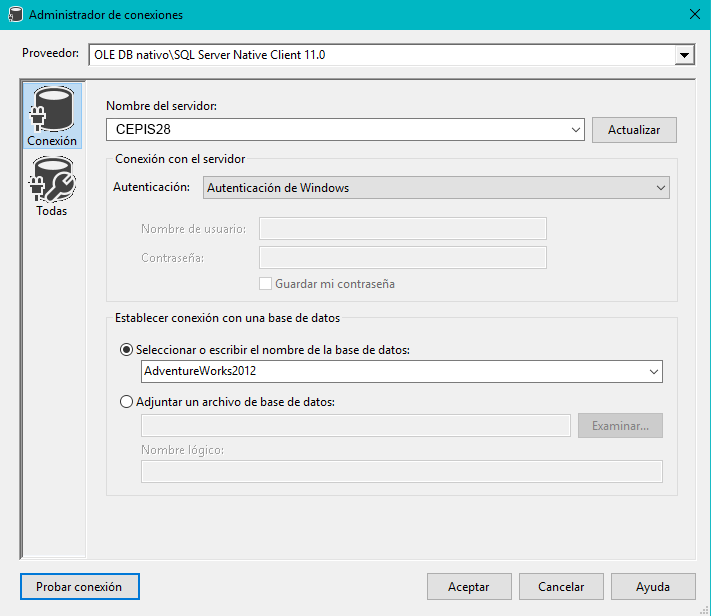
\includegraphics[width=14cm]{./Imagenes/tarea2_7}
	\end{center}

	\begin{center}
	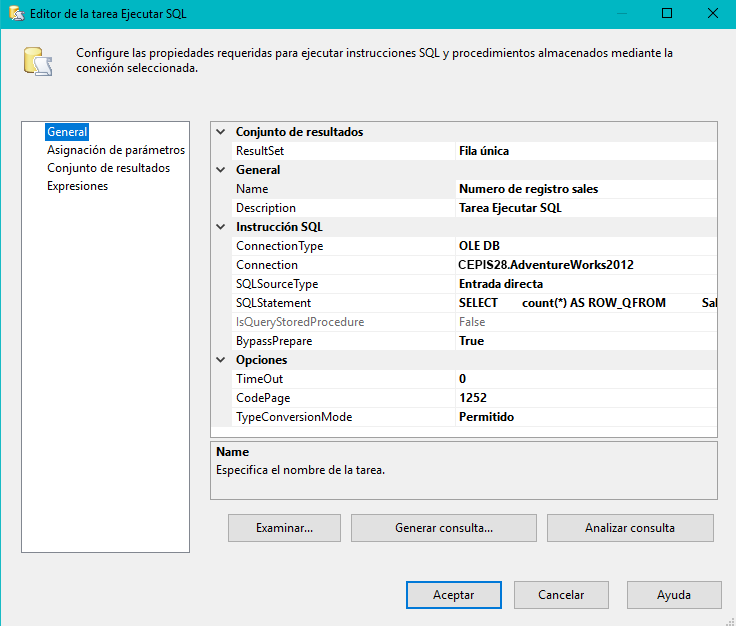
\includegraphics[width=14cm]{./Imagenes/tarea2_8}
	\end{center}

\item Editamos el componente Scrtipt Task Editor
\begin{center}
	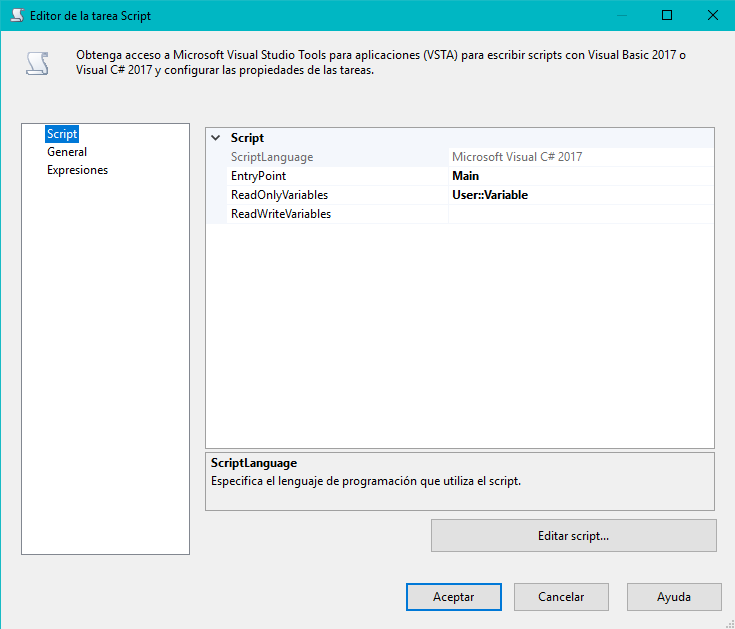
\includegraphics[width=14cm]{./Imagenes/tarea2_9}
	\end{center}

	\begin{center}
	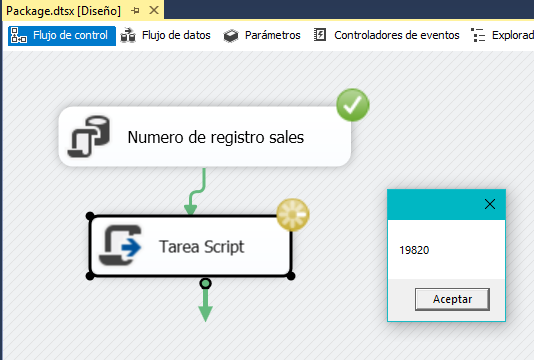
\includegraphics[width=14cm]{./Imagenes/tarea2_10}
	\end{center}
\begin{center}
	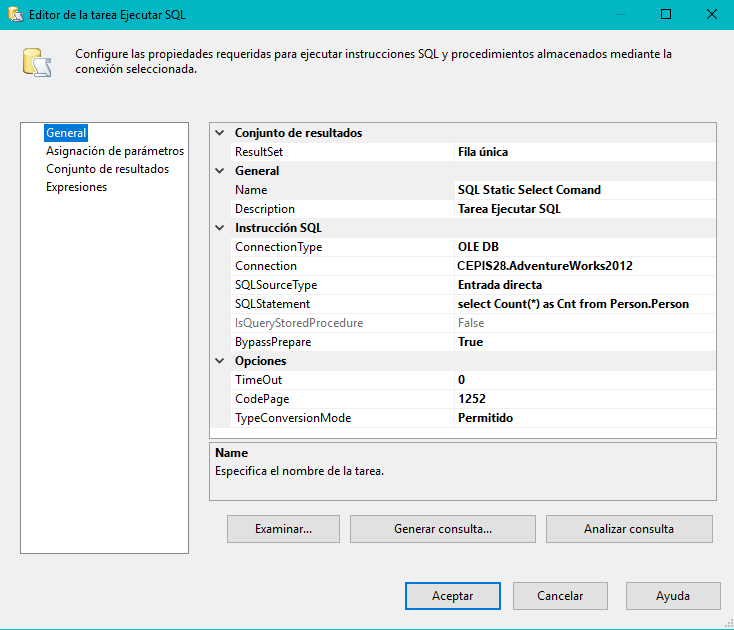
\includegraphics[width=14cm]{./Imagenes/tarea2_11}
	\end{center}

	\begin{center}
	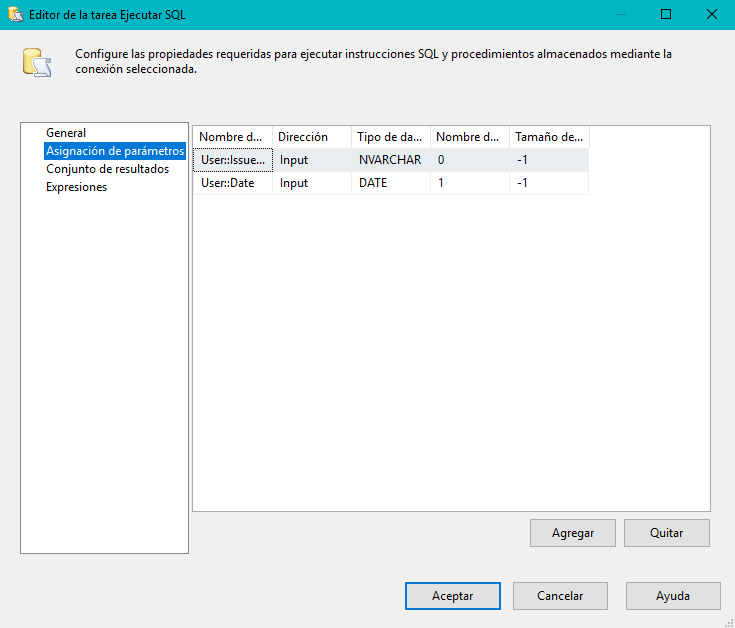
\includegraphics[width=14cm]{./Imagenes/tarea2_12}
	\end{center}

\begin{center}
	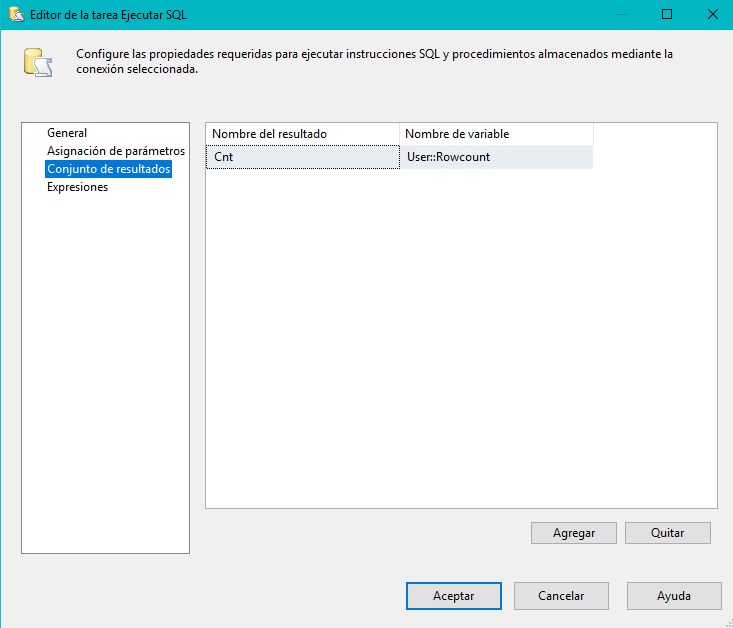
\includegraphics[width=14cm]{./Imagenes/tarea2_13}
	\end{center}

	\begin{center}
	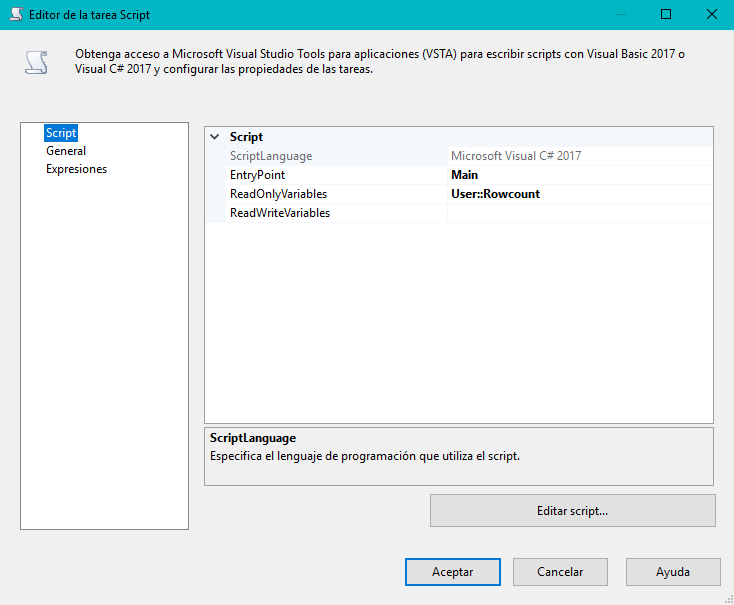
\includegraphics[width=14cm]{./Imagenes/tarea2_14}
	\end{center}

\item Guardamos y los ejecutamos.
   \begin{center}
	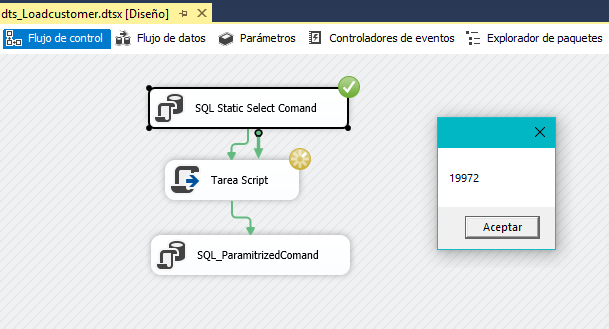
\includegraphics[width=14cm]{./Imagenes/tarea2_15}
	\end{center}



\end{itemize}
		